\documentclass[xcolor=dvipsnames]{beamer}
\usepackage[czech]{babel}
\usepackage[utf8]{inputenc}
\usepackage{graphics}
\usepackage{color}
\usepackage{amsfonts}
\usepackage{wrapfig}
\usepackage[export]{adjustbox}

\newcommand{\myuv}[1]{\quotedblbase #1\textquotedblleft}

\useinnertheme{rounded}
\definecolor{Favourite_colour}{HTML}{aa31aa}
\setbeamercolor{title}{fg=White,bg=Favourite_colour}
\setbeamercolor{frametitle}{fg=White,bg=Favourite_colour}

\begin{document}
	
	\title{\textsc{\huge{Typografia a publikovanie}}}
	\subtitle{\textsc{\small{Typografia, história a jej pravidlá}}}
	\author{\scriptsize{Dávid Bolvanský\\xbolva00@stud.fit.vutbr.cz}}
	\date{\scriptsize{29. apríl 2016}}
	\maketitle

\begin{frame}{\textsc{\large{Niečo o~typografií}}}
	\begin{center}
		Typografia je súhrn pravidiel, ktoré podporujú zrozumiteľnosť a čitateľnosť textu. Zjednodušene povedané, je to náuka o~písme, jeho vhodnom výbere, použití a forme.
	\end{center}
	\begin{figure}[ht]
		\begin{center}
			\scalebox{0.3}{
\includegraphics{typografia_main.eps}}
    		\caption{\textit{Typografia}}
		\end{center}
	\end{figure}
\end{frame}


\begin{frame}{\textsc{\large{Typografia a jej história}}}
		História západnej typografie sa datuje okolo roku 1450 v~súvislosti s~vynálezom kníhtlače v~Európe. Ďalších niekoľko storočí dochádzalo predovšetkým k~skvalitňovaniu tlačiarenských strojov vývojom nových písiem.
	\bigskip
	\begin{figure}[ht]
		\begin{center}
			\scalebox{0.15}{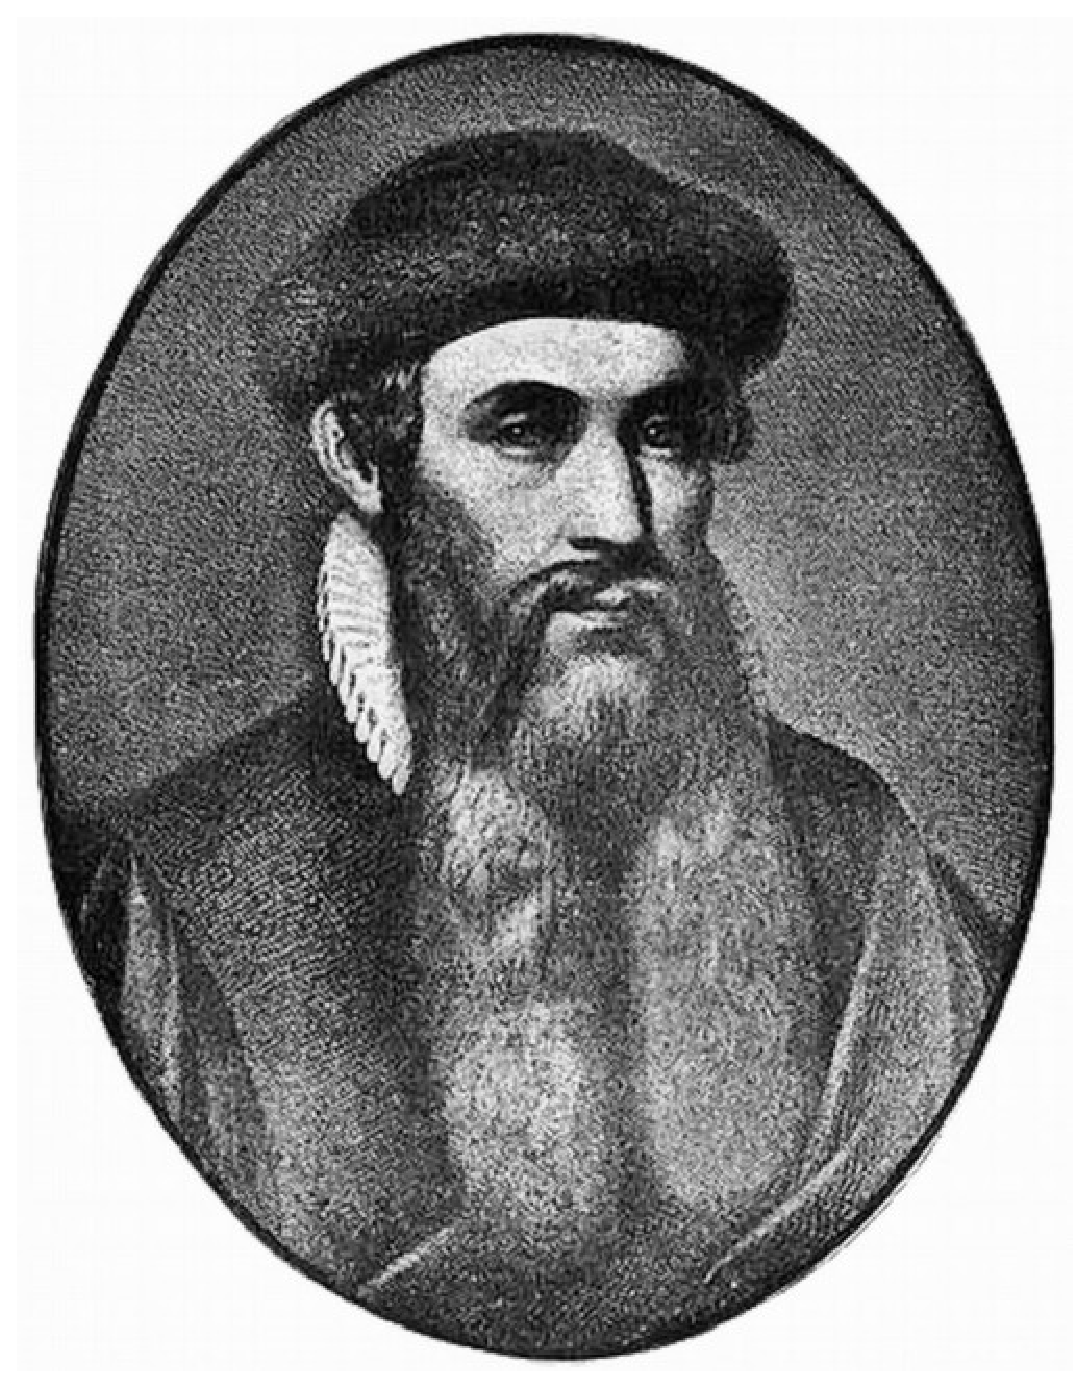
\includegraphics{gutenberg.eps}}
   			\caption{\textit{Vynálezca kníhtlače Johann Gutenberg}}
		\end{center}
	\end{figure}
	Najviac nových technólogií prichádza až v~20. storočí.
\end{frame}

\begin{frame}{\textsc{\large{Pravidlá, odporúčania a chyby v~typografií}}}
	Typografické pravidlá sú rovnaké a nezávisia od programu , ktorý používame na písanie a úpravu dokumentu.
    \bigskip
    \begin{figure}
	\begin{center}
    	\scalebox{0.5}{
\includegraphics[width=0.8\textwidth]{typografia.eps}}
    	\caption{Ukážka typografie}
    \end{center}
\end{figure}
\end{frame}


\begin{frame}{\textsc{\large{Vznik pravidiel}}}
	Pre písaný text sa postupom času vyvinulo veľké množstvo pravidiel, ktoré podporujú jeho zrozumiteľnosť a čitateľnosť.
  \begin{itemize}
  \bigskip
		\item Optický stred
		\item Zlatý rez
		\item Normalizované formáty
    	\item \emph{\textbf{\color{Favourite_colour}Čitateľnosť}}
	\end{itemize} 
\end{frame}

\begin{frame}{\textsc{\large{O systéme \LaTeX}}}
	\begin{itemize}
		\item {\LaTeX} je vysoko kvalitný typografický systém určený pre profesionálne a~poloprofesionálne sádzanie dokumentov 
        \item Bol vyvinutý v roku 1985 Leslie Lamportom 
		\item Ako sádzací nástroj používa program \TeX
        
        \item Základnou myšlienkou je, že autor dokumentu by sa mal starať len o~text článku. 
        \item O~formátovánie by sa mali postarať vývojári dokumentu
		
	\end{itemize}
\end{frame}

\begin{frame}{\textsc{\large{Zdrojový kód v \LaTeX e}}}
	\begin{figure}[ht]
		\begin{center}
			\scalebox{0.6}{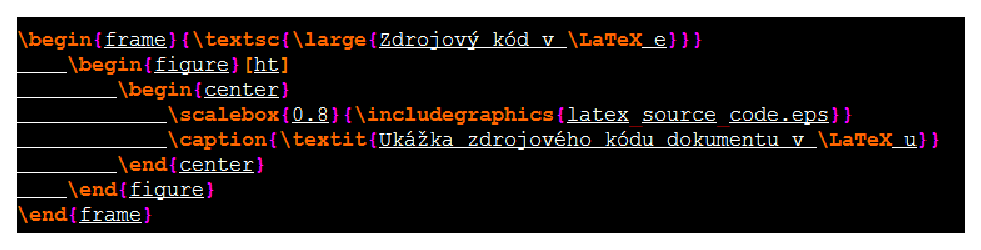
\includegraphics{latex_source_code.eps}}
    		\caption{\textit{Ukážka zdrojového kódu dokumentu v \LaTeX u}}
		\end{center}
	\end{figure}
\end{frame}


\begin{frame}{\textsc{\large{Zdroje}}}
  \begin{itemize}
  \bigskip
		\item Webové stránky o typografii
		\item Môj štvrtý projekt do predmetu \emph{\textbf{\color{Favourite_colour}Typografie a publikování}}
	\end{itemize} 
\end{frame}

\begin{frame}{\textsc{\large{Koniec}}}
	\vspace{\stretch{0.0075}}
	\centering
	\LARGE\textsc{Ďakujem za pozornosť.}
\end{frame}

\end{document}
